\documentclass[times, utf8,projekt]{fer}
\usepackage{booktabs}
\usepackage{amsmath}
\usepackage{hyperref}
\usepackage{titlesec}
\usepackage{graphicx}
\usepackage{xurl}
\graphicspath{{figures/}}
\PassOptionsToPackage{hyphens}{url}\usepackage{hyperref}
\begin{document}

% TODO: Navedite broj rada.
%\thesisnumber{000}

% TODO: Navedite naslov rada.
\title{Umjetna inteligencija u adaptivnom učenju}

% TODO: Navedite vaše ime i prezime.
\author{Jelena Nemčić, Marin Ovčariček,Zvonimir Sučić,Ivana Žeger}

\maketitle
% stranice s napomenom o umetanju izvornika rada. Uklonite naredbu \izvornik ako želite izbaciti tu stranicu.
%\izvornik
% Dodavanje zahvale ili prazne stranice. Ako ne želite dodati zahvalu, naredbu ostavite radi prazne stranice.
%\zahvala{}
%\tableofcontents
%Dodati općenitu ideju projekta
\chapter{Uvod}
Adaptivno učenje u e-learning softverima tipično funkcionira tako da mjeri razinu znanja korisnika kroz početni skup pitanja, virtualnu simulaciju i/ili dodijeljene zadatke. Na temelju podataka prikupljenih iz odgovora korisnika, takav softver u stvarnom vremenu procjenjuje razliku između korisničkog znanja i znanja potrebnih za određenu kompetenciju, te odabire lekcije i zadatke za korisnika tako da minimizira količinu edukacijskog sadržaja koji tom korisniku prikazuje.\newline
Konstrukcija algoritma za određivanje puta za adaptivno učenje tipično se radi na dva načina: 1) kreiranjem formalnog modela znanja za određenu domenu, a koji kreiraju eksperti iz te domene ili 2) koristeći algoritamski pristup baziran na teorijama Bayesian Knowledge Tracing i Item Response Theory koji na temelju odgovora polaznika edukacije procjenjuje vjerojatnost da je polaznik usvojio određenu vještinu/koncept (što ponovno zahtijeva unaprijed definirane vještine/koncepte).\newline
U posljednje vrijeme, a s obzirom na dostupnost sve većih količina podataka (big data) ponovno su oživjele i dodatno se razvijaju tehnologije kreiranja grafova znanja (npr. pomoću dubokog učenja), a koji s obzirom na to da su kreirani statistički mogu biti mnogo kompleksniji i uže segmentirani (precizniji) u odnosu na one koje kreiraju eksperti nekog područja. Dodatno, prikupljanje velike količine informacija u različitim domenama omogućuje da kreiranje grafova znanja ne bude ograničeno samo na one tvrtke koje imaju golem broj korisnika kao što su Google ili Facebook). Na temelju inicijalnog istraživanja vjerujemo da se ova metoda može primijeniti i na kreiranje grafova znanja za adaptivno učenje, te time omogućiti s jedne strane znatno veću adaptivnost, a s druge strane veću jednostavnost kreiranja takvih grafova.\newline
Ovo je posebno važno za područja edukacije izvan formalnog obrazovanja, gdje nisu strogo definirane ishodi učenja i testovi kojima se mjeri je li neki ishod učenja dostignut kod pojedinog polaznika. Dva primjera za to su instrukcije, gdje učeniku često nedostaju i predznanja iz drugih područja koje je ranije u školi trebao usvojiti, te korporativne edukacije, koje često obuhvaćaju ljude različitih struka i različitim znanjima iz domene za koju nastoje dobiti certifikat.


\chapter{Cilj i postupak}
Stoga je cilj ovog projekta provjeriti sljedeće:
\begin{itemize}
\item Provjera mogućnosti kreiranja grafa znanja isključivo na temelju točnosti odgovora na zadacima iz jedne domene znanja koje korisnici daju i informacije o redoslijedu zadavanja zadataka pojedinom korisniku
\item Ako je navedeno moguće, potrebno je provjeriti može li se kreirati graf znanja na temelju rješavanja zadataka za istu domenu na temelju parcijalnog broja zadataka (što realnije reprezentira dostupne zadatke za stvarne domene – rijetko su dostupna baš sva znanja iz neke domene da bi se mogla kreirati zadaci koji pokrivaju baš svaku informaciju u toj domeni)
\item Ako je navedeno moguće, potrebno je provjeriti može li se isto napraviti i za neku domenu realnog znanja\newline
\end{itemize}
Ukratko, ovim se projektom provjerava može li se graf znanja potreban za adaptivno učenje kreirati metodama dubokog učenja na temelju ponašanja korisnika na zadacima (probabilistički), a bez potrebe za time da eksperti unaprijed određuju koncepte/vještine u koje se grupiraju zadaci ili čak sam graf znanja.\newline\newline
Za potrebe ove provjere kreirat će se:
\begin{itemize}
	\item umjetni, zatvoreni graf znanja 
	\item zadaci koji pokrivaju sve informacije prisutne u tom zatvorenom grafu znanja\newline
\end{itemize}
Potom će se zadaci dati testerima na rješavanje, tako da se:
\begin{itemize}
	\item varira redoslijed zadataka koje pojedini tester dobiva kako bi pokrio sve kombinacije
	\item bilježi točnost odgovora testera na zadatak
	\item u slučaju netočnog odgovora testeru se prikazuje točna informacija.
\end{itemize}

\chapter{Bayesian knowledge tracing (BKT)}
\label{ch:BKT}
\section{Općenito o BKT}
Bayesian Knowledge Tracing koristi Hidden Markov Model i ima 4 osnovna parametra:
\begin{itemize}
	\item p(L0) - vjerojatnost da je korisnik a priori savladao gradivo
	\item p(G) - vjerojatnost da je korisnik pogodio točan odgovor bez da ima potrebno znanje	
	\item p(S) - vjerojatnost da je korisnik krivo odgovorio iako ima potrebno znanje	
	\item p(T) - vjerojatnost da je znanje prešlo iz NE ZNA u ZNA nakon prilike da se primjeni znanje
\end{itemize}
Kao izlaz dobivaju se vrijednosti:
\begin{itemize}
	\item p(L) - vjerojatnost ovladavanja vještinom (eng. probability of skill mastery)
	\item p(C) - vjerojatnost da će korisnik ispravno primijeniti vještinu u budućnosti (eng. probability of the student correctly applying the skill on a future practice)\newline
\end{itemize}

\begin{equation}
 p(L_t\mid obs=correct)=\frac{p(L_t)*(1-p(S))}{p(L_t)*(1-p(S)+(1-p(L_t)*p(G))}
\end{equation}\newline
\begin{equation}
 p(L_t\mid obs=wrong)=\frac{p(L_t)*p(S)}{p(L_t)*p(S)+(1-p(L_t)*(1-p(G))}
\end{equation}\newline
\begin{equation}
 p(L_{t+1})=p(L_t\mid obs=correct) + (1-p(L_t\mid obs=correct))*p(T)
\end{equation}\newline
\begin{equation}
 p(C_{t+1})=p(L_{t+1}) * (1-p(S)) + p(L_{t+1})*p(G)
\end{equation}

\section{Ideje}
Prvobitna ideja je bila da se p(L0) računa iz inicijalnih pitanja, vrijednosti p(G) i p(S) bi se prema preporuci iz rada(trebalo bi pronaći kojeg i baciti referencu) stavile na interval [0,0.3], [0,0.1] te bi se p(T) postavio prema preporuci eksperta što ne želimo jer je cilj ovog projekta da smanjimo zadatke eksperata na minimum.\newline
To je ukazalo na potrebu pronalaska algoritama koji bi uz pomoć nekog skupa podataka aproksimirali parametre za BKT.
\section{Problemi i zadaci}
\begin{itemize}
	\item proučiti parametar p(T)
	\item proučiti kodove sa githuba kako bi se dobila ideja kako algoritam funkcionira
	\item napraviti malu implementaciju s malo pitanja i provjeriti radi li
	\item proučiti parameter fitting uz pomoć EM algoritma, stohastic gradient descenta ili neke druge metode
	\item kako napraviti input dataset, prikupiti podatke
	
	
\end{itemize}
\section{Dobivanje BKT parametara}
\subsection{EM (expectation-maximization) algoritam}

\begin{itemize}
	\item iterativni algoritam za pronalaženje (aproksimiranje) najveće izglednosti (eng. maximum likelihood) ili maksimalne a posteriori (MAP) procjene parametara u statističkim modelima
	\item model ovisi o nepoznatim latentnim varijablama
	\item EM iteracija sadrži 2 koraka:
	\begin{itemize}
		\item 	korak očekivanja (E), koji stvara funkciju za očekivanje log-izglednosti koja se procjenjuje pomoću trenutne procjene parametara, procjenjuju se vrijednosti latentnih varijabli
		\item 	korak maksimizacije (M), koji izračunava parametre distribucije koji maksimiziraju očekivanu log-izglednost pronađenu u E koraku, ti se parametri zatim koriste za procjenu latentnih varijabli u sljedećem E koraku
	\end{itemize}
	
	\item primjenjuje se kada želimo odrediti parametre distribucije (normalna, eksponencijalna, …)
	\item problem: za korištenje potrebo znati distribuciju podataka ili točne vrijednosti (eng. true values) traženih parametara
	
\end{itemize}
Kroz ovo istraživanje nije pronađena niti jedna implementacija EM algoritma za aproksimaciju BKT parametara niti je napravljena vlastiti implementacija zbog prevelikog praga znanja matematike.

\subsection{Grid search i Simulated Annealing}
Pronađen je kod napisan u Javi koji računa BKT parametre tehnikom simuliranog kaljenja \url{https://github.com/wlmiller/BKTSimulatedAnnealing}. U README na githubu se također spominjao kod koji je bio baza za to, on je koristio običan grid search kako bi izračunao parametre. Oba koda su prevedena u python i prilagođena našim skupovima podataka. Na kraju se ispostavilo da je "simulirano kaljenje" povoljnije te se grid search odbacio.
\section{Rezultati}
\begin{itemize}
	\item napravljen google forms kviz sa 20 pitanja iz biologije, ispitanici moraju odgovoriti na svih 20 pitanja kako bi podaci ušli u dataset
	\item napravljena python skripta koja pretvara podatke dobivene iz google formsa u oblik prikladan za treniranje BKT-a i pronalaženje parametara
	\item pronađen je kod u Javi koji tehnikom simuliranog kaljenja aproksimira parametre za BKT uz pomoć danog dataseta, kod je preveden u python skript
	\item napravljena python skripta za BKT koja određuje vjerojatnost da je ispitanik naučio/  savladao gradivo
	\item uz pomoć skripte za aproksimaciju BKT parametara, nađene su njihove vrijednosti za svaku vještinu iz ASSISTMENTS dataseta i pohranjenje u google sheets tablicu
	\item dobiveni parametri algoritmom simuliranog kaljenja uspoređeni su s onima dobivenima pomoću grid search metode -> vrijednosti parametara su skoro iste, vrlo male razlike
	\item napravljen google forms kviz sa po 6 pitanja iz 5 koncepata, izračunati su parametri za taj dataset
	\item BKT kod i kod za aproksimaciju BKT parametara su se dalje koristili u bilježnicama za izgradnju grafa probabilističkim metodama
	
\end{itemize}
\section{Poveznice}
\subsection{BKT}
\url{https://en.wikipedia.org/wiki/Bayesian_Knowledge_Tracing}\newline
\url{http://www.cs.cmu.edu/~./ggordon/yudelson-koedinger-gordon-individualized-bayesian-knowledge-tracing.pdf}\newline
\url{https://github.com/CAHLR/pyBKT/blob/master/README.md}\newline
\url{https://www.learnlab.org/uploads/mypslc/publications/bca2008v.pdf}\newline
\url{https://www.upenn.edu/learninganalytics/ryanbaker/paper_143.pdf}\newline
\url{https://github.com/yemao616/Bayesian-Knowledge-Tracing}\newline
\url{http://www.cs.cmu.edu/~./ggordon/yudelson-koedinger-gordon-individualized-bayesian-knowledge-tracing.pdf}\newline
\url{https://www.fi.muni.cz/~xpelanek/publications/umuai-overview.pdf}\newline
\url{https://medium.com/@joyboseroy/modelling-a-students-learning-34375b0131dd}\newline
\url{https://www.math.vu.nl/~sbhulai/publications/data_analytics2018c.pdf}\newline
\subsection{Pronalaženje parametara}
\url{https://www.fmrib.ox.ac.uk/datasets/techrep/tr00yz1/tr00yz1/node9.html}\newline
\url{https://github.com/wlmiller/BKTSimulatedAnnealing/blob/master/computeKTparams_SA.java}\newline
\url{https://www.upenn.edu/learninganalytics/ryanbaker/paper_143.pdf}\newline
\url{https://educationaldatamining.org/files/conferences/EDM2018/papers/EDM2018_paper_14.pdf}\newline
\url{http://yudelson.info/hmm-scalable/}\newline
\url{https://www.educationaldatamining.org/EDM2015/proceedings/short364-367.pdf}\newline
\url{https://concord.org/wp-content/uploads/2016/12/pdf/tracking-student-progress-in-a-game-like-learning-environment.pdf}\newline
\url{https://tinyheero.github.io/2016/01/03/gmm-em.html}\newline
\url{https://machinelearningmastery.com/expectation-maximization-em-algorithm/}\newline
\url{http://rstudio-pubs-static.s3.amazonaws.com/1001_3177e85f5e4840be840c84452780db52.html}\newline
\url{https://www.colorado.edu/amath/sites/default/files/attached-files/em_algorithm.pdf}
\chapter{Bayes graf}
	\section{Uvod}
	
	Ideja je napraviti vlastiti model koji iz skupa podataka računa vjerojatnost savladavanja koncepata te se prema njima gradi graf znanja.\newline
	Prvi pristup je račun uvjetnih vjerojatnosti $p(Y_j\mid X_i)$, odnosno vjerojatnost da korisnik zna (savladao je) koncept Y ako zna X. Koristi se klasična formula Bayesove uvjetne vjerojatnosti čime se gradi matrica odnosa koncepata.
	\begin{equation}
		p(Y \mid X)=\frac{p(X \wedge Y)}{p(X)}
	\end{equation}
	\newline Vjerojatnost Y uz X nam govori koliko je poznavanje X bitno za poznavanje Y. Pretpostavka je da će korisnik s većom vjerojatnošću znati jednostavniji koncept ako zna kompliciraniji (nadogradnju jednostavnog), ako su X uz Y i Y uz X podjednaki (potreban je neki prag) može se pretpostaviti da su koncepti nezavisni ili bi se mogli spojiti kao jedan koncept. \newline
	Drugi pristup je bio pokušaj da se gleda kad su koncepti X i Y točni s obzirom koji od njih je položen prvi, pretpostavka je bila da bi se tako mogla odrediti relacija nadogradnje, odnosno prethodnika. Pristup nije uspio jer ili nije moguć ili nije bio dobro definiran / implementiran.\newline
	Najveći problem u oba pristupa je to što pokušavamo dobiti ovisnosti među konceptima,a ne pitanjima. Za razliku od pitanja za koncepte se ne može reći da ih se zna/ne zna jer se oni sastoje od više pitanja te se može samo gledati postotak riješenosti za svakog studenta / prosječan postotak riješenosti. Prosječan postotak rješenosti se može gledati kao pripadnost neizrazitom skupu ZNA odnosno 1- postotak riješenosti kao pripadnost skupu NE ZNA, to komplicira stvari kod Bayesovog zaključka. Potrebno je pronaći/proučiti postoji li ekvivalent Bayesovog zaključka kada se koriste neizraziti skupovi odnosno kontinuirane vrijednosti [0,1].
	
	\section{Problem kontinuiranih vrijednosti}
		Običan Bayesov zaključan radi sa diskretnih vrijednostima (true/false, 1/0). Dok je to istina kod izračuna vjerojatnosti i točnosti pitanja, isto se ne može reći za koncepte. Može se gledati da je koncept položen s nekom vjerojatnošću ili da određen pokušaj ispita pripada skupo "položen" s nekom pripadnošću, to je obično postotak točnih bodova i to je racionalan broj. Iako postoji Bayesov zaključak za kontinuirane vrijednosti nije jednostavan za izračunati jer se teško mogu dobiti latentne razdiobe bodova za neku populaciju. Pošto je Bayes kontinuiranoj domeni prekompliciran za računati potražena je altrenativa te se došlo do zaključka da se treba nekako vratiti u diskretnu domenu, odnosno napraviti model koji može odlučiti kad neki koncept je ili nije položen.\newline
		Najjednostavnije rješenje je ručno za svaki koncept zadati bodovni prag te bi svi korisnici koji zadovolje prag imali oznaku da su savladali koncept. To i nije najbolji pristup jer se ne uzimaju u obzir razne druge varijable kao što su npr. vjerojatnost da korisnik pogađa ili slučajno pogrješi.\newline
		Kako bi se rješio taj problem, pronađena je tehnika Bayesian Knowledge Tracing~\ref{ch:BKT} i kombinirana sa vlastitom tehnikom raspodjele po Gaussu kako bi se bolje aproksimiralo trenutno znanje korisnika.
	\section{Skaliranje korisnika prema Gaussu}
		Kao alternativa BKT-u implementirano je skaliranje studenata prema Gaussu:
	\begin{itemize}
		\item za svakog studenta i za svaku vještinu izračunat je percentil kojemu taj student pripada u ovisnosti o odgovorima svih studenata
		\item postavi se threshold koji odgovara percentilu iznad kojeg se nalaze studenti koji su položili vještinu\newline
	\end{itemize}
		Paralelno se za svakog studenta računa prolaznost (0 ili 1) prema BKT-u i prema Gaussu:
	\begin{itemize}
		\item ako se one poklapaju, to se uzima kao vrijednost za tog studenta
		\item ako je zbroj te dvije jačine veći od 0, uzima se da je student položio vještinu
		\item ako su različite gleda se jačina s kojom model tvrdi da je student pao/položio, ona se računa na sljedeći način:%dodati sliku ispod
	\end{itemize}
	
		
		
		
	
		 
		
		%TREBA UBACITI SLIKU

		
	\section{Izvještaji}
		\subsection{22.07.2020.}
		\textbf{Planovi, problemi:}
		\begin{itemize}
			\item pronaći dobru vrijednost za cutoff kod micanja poveznica kod grafa
			\item iteriranje po retcima dataframeova - nije dobro, treba pronaći efikasnije načine obrade tablica
			\item isprobati program na malom datasetu
			\item isprobati program na biologija dataset, ali gledajući da je svako pitanje jedan koncept (napraviti i program koji bi pretvorio pitanja u koncepte)
			\item proučiti librarye za crtanje usmjerenih grafova (boje, labele, debljine poveznica)
			\item dopuniti program da crta usmjerene grafove
			\item pokušati naći implementacije EM i grid search algoritma za računanje BKT parametara
			\item pokušati pronaći dobro objašnjenog bayesa u kontinuiranoj domeni
			\item pronaći naprednije implementacije BKT-a koje uzimaju više parametara
			\item osmisliti strukture podataka koje bi predstavljale čvorove i povezivale pitanja,koncepte i ostale čvorove u jednu cjelinu, omogućavale obilazak grafa te nalaženje najkraćeg puta (po nekom kriteriju) od početnog do ciljnog čvora
			\item napraviti novi test koji bi imao mali broj pitanja iz različitih područja koja su međusobno povezana (npr. stanica, što je to -> građa stanice -> građa različitih organela) i na tome isprobati program\newline
		\end{itemize}
		\textbf{Rezultati}
		\begin{itemize}
			\item napravljena skripta za izgradnju grafa pomoću uvjetnih vjerojatnosti i Bayesove formule
			\begin{itemize}
				\item ulaz: datoteka koja sadrži BKT parametre za sve vještine i datoteka koja sadrži tablicu studenata i njihovih odgovora
				\item izlaz: matrica koja predstavlja matricu susjedstva grafa, gdje svaki element predstavlja “jačinu”/”vjerojatnost” s kojom je koncept \textit{i} povezan s konceptom \textit{j}
				\item skripta sadrži razred BKT i funkcije za računanje vjerojatnosti p(X), računanje zajedničke vjerojatnosti p(X and Y) i računanje matrice ovisnosti
			\end{itemize}
			\item skripta je isprobana na dosad prikupljenim podacima testa za biologiju (74 odgovora) i dobiveni su realni rezultati, ali nismo imali sa čime usporediti budući da je to samo jedan koncept
			\item izrađeni su grafovi na malom umjetnom datasetu i datasetu biologija gdje su se pitanja gledali kao zasebni koncepti
			\item za potrebu prilagodbe pitanja u koncept napravljena je skripta koja uzima pitanja kao koncepte, računa vjerojatnosti te crta graf
			\item za crtanje grafova koristio se netowrkx library
			\item vrijednost cutoffa za izgradnju grafova bi prema procjeni trebala u intervalu [0.8,0.95]. Nismo našli nikakve službene izvore/preporuke tako da  će se za sada cutoff morati ručno procijeniti.
			\item odrađena optimizacija koda gdje se boljim iteriranjem po dataframeu dobiva ljepši i brži kod, daljnja optimizacija je vjerojatno moguća, ali trenutno nije prioritet trošiti vrijeme na istraživanje kako to napraviti
		\end{itemize}
		\subsection{28.07.2020.}
		\begin{itemize}
			\item napravljen je je novi kviz sa pet koncepata iz biologije
			\item svaki koncept ima 6 pitanja
			\item problemi: kviz ima više pitanja nego prošli, u prosjeku je mentalno zahtjevniji, znanje koncepta vjerojatno nije dobro pokriveno sa tih 6 pitanja, neki koncepti su su značajno zahtjevniji nego drugi te raspodjela pitanja po težini nije ista u svakom konceptu i vjerojatno nije optimalna budući da se trenutno svi odgovori vrednuju jednako
			\item u trenutku pisanja izvještaja imamo samo 25 odgovora na kviz, pokrenuli smo model da vidimo kako reagira na manjak podataka
			\item rezultati su očekivano lošiji nego prije, u početku su od 5 koncepata na grafu bila prikazana samo 3 te smo dobili NaN vrijednosti matrici povezanosti, što se dogodilo jer prema pragu BKT-a niti jedan student nije položio predmet te se pojavilo dijeljenje sa nulom. Nakon što smo spustili prag prolaska sa 0.95 na 0.9, pojavio se dodatan čvor na grafu i nismo imali NaN, ovo ukazuje na problem osjetljivosti BKT-a na manjak podataka i na redoslijed točno/netočno odgovora studenata
			\item također same povezanosti grafa nisu imali smisla (npr. da je živčana stanica preduvjet za diobu stanice)
			\item ovi rezultati nisu iznenađujući jer je samo svojstvo BKT-a da je osjetljiv na redoslijed i uzastopno ponavljanje točno/netočno u nizu odgovora te su modeli bazirani na vjerojatnostima jako osjetljivi na manjak ulaznih podataka
			\item IDEJA: isprobati jednostavno skaliranje bodova studenata na temelju Gaussove raspodjele te odrediti prag prema kojem bi se dijelili na prolazak/pad. Ovako bi se maknula loša svojstva BKT-a, ali bi model postao još jednostavniji te bi vjerojatno imao slabija svojstva predviđanja.
			\item treba proučiti kako napraviti da linije povezanosti imaju različite debljine s obzirom na jačinu povezanosti, onda bi se mogao malo spustiti cutoff da se dobije bolji pregled ovisnosti između koncepata
		\end{itemize}
		\begin{figure}[!htb]
		\centering
		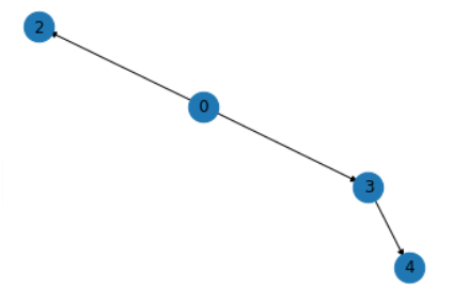
\includegraphics[scale=1]{Bayes_graf3.png}
		\caption{}
		\label{}
		\end{figure}
		Legenda:
		
		0: Stanica
		1: DNA
		2: Stanični metabolizam
		3: Dioba stanice
		4: Živčana stanica

		\subsection{29.07.2020.}
		\begin{itemize}
			\item napravljen program koji generira proizvoljan umjetan dataset
			\item obavezni ulazni argumenti su broj studenata i trojka (broj pitanja po konceptu, prosječni udio točnih odgovora u tom konceptu, standardna devijacija)
			\item skripta pretpostavlja da svaki student odgovara na sve koncepte i na sva pitanja
			\item prema gaussovoj raspodjeli svakog koncepta se svakom studentu pridjeljuje postotak točno riješenih zadataka te mu se prema toma generiranju rješenja
			\item dataset se sprema u klasičnom obliku kojeg naše skripte za crtanje mogu koristiti
			\item u trenutku pisanja ima 75 odgovora na novu anketu
			\item pokrenuta je obrada podataka i izračunavanje bkt parametara za trenutne odgovore
			\item cutoff threshold je 0.5
		\end{itemize}
		\begin{figure}[!htb]
			\centering
			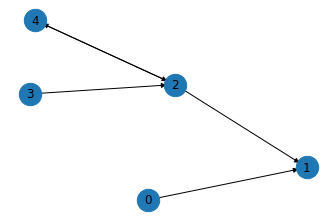
\includegraphics[scale=1]{Bayes_graf4.png}
			\caption{}
			\label{}
		\end{figure}
		Legenda:
		
		0 : Stanica
		1 : DNA
		2 : Živčana stanica
		3 : Stanični metabolizam
		4 : Dioba stanice\newline
		\newline Zaključci: ljudi koji su znali diobu stanicu i stanični metabolizem generalno su znali i živčanu stanicu, ljudi koji su znali diobu stanice obično su znali i živčanu stanicu te ljudi koji su znali DNA su obično znali i stanicu/živčanu stanicu. Ovo ne prikazuje realan slijed učenja biologije, ali nije ni očekivano da prikazuje jer biologija nema tako strogi uvjetni slijed koncepata kao npr. matematika\newline
		\newline \textbf{Rezultati umjetnih datasetova}	\newline
		BKT-annealing daje predzadnjem konceptu jako male vrijednosti parametara zbog čega nitko ne prolazi taj predmet, dobivaju se NaN vrijednosti te se ne crta taj čvor.
		\begin{figure}[!htb]
			\centering
			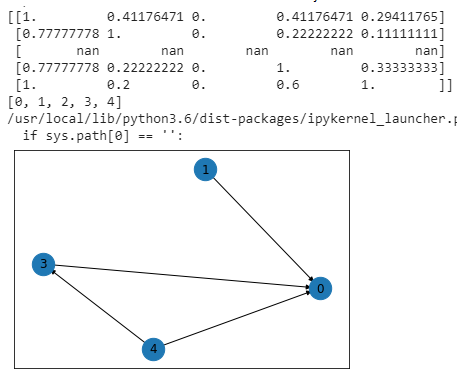
\includegraphics[scale=1]{Bayes_graf6.png}
			\caption{}
			\label{}
		\end{figure}
		Ovo ukazuje na veliku osjetljivost aproksimacije parametara na broj i redoslijed točnih odgovora studenata, ovo se može poboljšati pažljivim odabirom mean i stddev vrijednosti kod generiranja umjetnog dataseta (ne odabrati premali mean te pogotovo ne uzimati veliki stddev kod malog meana i uz mali broj studenata jer se može dogoditi da većina njih dobije male postotke riješenih zadataka što daje loše bkt parametre). Drugi način je staviti nekakvo zaglađivanje kako bi se onemogućilo dobivanje NaN vrijednosti s nekom malom konstantom (ovo samo sprječava errore, ali ne pomaže u točnosti modela). Zadnje što ostaje je pronaći i razviti alternativu BKT-u koja nije toliko osjetljiva.
		\subsection{30.07.2020.}
		\begin{itemize}
			\item 	ideja: trenutno je za model potrebno da svi studenti rješavaju sve koncepte, to nije pojava u realnim skupovima podataka pa se predlaže sljedeće rješenje - kod računa joint\_probabilitya uzeti presjek studenata koji su rješavali koncept A i koncept B po njihovom student\_id-u, sam izračun pX se ostavi kao što je i bio. Ova pretpostavka bi mogla vrijediti jer ako je realan skup podataka dovoljno velik te ako je presjek također dovoljno velik oni će imati dovoljno informacije da se da realni prikaz ovisnosti između koncepata
			\item ideja2: iako je bitno da studenti odgovaraju istim redoslijedom na pitanja taj uvjet se može izbjeći naknadnim sortiranjem po quesiton\_id-u. Ovo nije prioritet za implementirati jer gotovo svi standardizirani ispiti daju pitanja istim redoslijedom te daju svakom studentu ista pitanja (treći uvjet za funkcioniranje modela)
			\item ideja3: napraviti skriptu iz koja bi bila skup svi do sad proizvedenih skripti. Ta skripta bi zapravo bila skup “main” funkcija dobivenih pozivanjem određenih funkcija iz  ostalih bilježnica (ovdje se radi importanje, a ne kopiranje postojećeg koda)
			\item Mogućnosti sjedinjene skripte:
			\begin{itemize}
				\item Izgradnja grafa
				\item Generiranje umjetnog dataseta
				\item BKT simulated annealing
				\item Obrada podataka s google formsa
				\item Gledanje pitanja kao koncepata
			\end{itemize}
		\end{itemize}
	
		\subsection{31.07.2020.}
		\begin{itemize}
			\item napravljene su potrebne izmjene skripti kako bi se broj studenata na pojedinim vještinama mogao razlikovati, što više odgovara realnim podacima (neće svaki student odgovarati na pitanja iz svake vještine)
			\item kod računanja vrijednosti joint\_probability uzima se presjek studenata koji su rješavali koncept A i koncept B (gleda se njihov student\_id) i računa njihova uspješnost
			\item kod generiranja umjetnog dataseta dodan je parametar broj\_studenata za svaki koncept
			\item napravljena je skripta koja sjedinjuje sve važne dosad napravljene skripte u niz funkcija koje se lako pozivaju
			kako bi se moglo raditi importanje .ipynb fileova potrebno je u istom kazalu gdje su  fileovi dodati praznu \_\_init\_\_.py datoteku
			\item 	dodana je mogućnost odabira pragova cutoffa, gaussa, bkt-a kod pozivanja funkcije build\_graph().
			\item 	trenutna greška u skripti pitanja->koncepti, izračun pX-a se pokreće dva puta, prvi put je sve u redu dok se drugi put neki keyevi ne nalazi u dictionaryu, uzrok tome je drugi poziv funkcije calculate, kod splitanja se maknu neki indeksi, greška je u pisanju koda, svugdje se gleda range(noStudents) umjesto list studenata, kod kfolda se određeni studenti miču i ostaju samo neki id-ovi i noStudents se smanjuje i može se desiti npr. da se makne student s id-om 1 što znači da ga više nema u dictionaryju ali for petlja će ga i dalje pokušati dohvatiti, treba napisati program da radi prema student id-u, ako se ne nađe bolje rješenje maknut će se k-fold izračun jer trentna implementacija nije dobra - POPRAVLJENO
			\item 
			treba u oba crtanja grafa riješiti problem dijeljenja sa nulom - DJELOMIČNO POPRAVLJENO - radi, ali rješenje nije najbolje (ako pX bude nula, ne dijeli se nego se joint probability postavlja na 0)
			\item taj kod bi se možda mogao koristiti kao provjera povezanosti pitanja
			\item zadnje što preostaje nakon popravljanja i uljepšavanja koda koji pretvara pitanja u koncepte jest smisliti obradu google formsa tako da je omogućeno da bude različit broj pitanja po konceptu, s tim da su pitanja grupirana odnosno nisu pomiješana po ispitu
		\end{itemize}	
		\subsection{14.08.2020.}
			Prebačene su skripte iz colaba u .py fileove na git, obavaljeno refaktoriranje kako bi se malo više standardizirale konvencije imenovanja i ostala uljepšavanja koda.Napravljena main skripta koju se lagano može programirati da radi razne operacije uz pomoć funkcija koje pozivaju importane module.
	\section{Poveznice}
	\url{https://ocw.mit.edu/courses/mathematics/18-05-introduction-to-probability-and-statistics-spring-2014/readings/MIT18_05S14_Reading13a.pdf}\newline
	\url{https://www.probabilitycourse.com/chapter9/9_1_2_MAP_estimation.php}\newline
	\url{https://www.sciencedirect.com/science/article/abs/pii/S0951832017300674}\newline
	\url{https://arxiv.org/pdf/1610.09156.pdf}\newline
	\url{http://www.dia.fi.upm.es/~mgremesal/MIR/slides/Lesson\%206\%20(Inference\%20from\%20Conditional\%20Fuzzy\%20Propositions).pdf}\newline
	\url{https://www.intechopen.com/books/fuzzy-logic/some-methods-of-fuzzy-conditional-inference-for-application-to-fuzzy-control-systems}
\chapter{Zaključak}
Zaključak.
\bibliography{literatura}
\bibliographystyle{fer}

\begin{sazetak}
Sažetak na hrvatskom jeziku.

\kljucnerijeci{Ključne riječi, odvojene zarezima.}
\end{sazetak}

% TODO: Navedite naslov na engleskom jeziku.
\engtitle{Title}
\begin{abstract}
Abstract.

\keywords{Keywords.}
\end{abstract}

\end{document}

% TODO: Ne radi bibtex,jel mi treba?